\documentclass[tikz,border=5pt]{standalone}
\usepackage{amsmath}
\usetikzlibrary{arrows.meta,calc,positioning,shapes.geometric,shapes.symbols}

\definecolor{skyblue}{RGB}{225,241,250}
\definecolor{groundgreen}{RGB}{225,239,218}
\definecolor{accessblue}{RGB}{31,119,180}
\definecolor{interferencered}{RGB}{205,55,48}
\definecolor{backhaulgreen}{RGB}{42,135,95}
\definecolor{uavorange}{RGB}{229,138,46}
\definecolor{darkgray}{RGB}{70,75,82}

\tikzset{
  access/.style={accessblue, line width=0.9pt},
  interference/.style={interferencered, dashed, line width=0.9pt},
  backhaul/.style={backhaulgreen, densely dashed, line width=1.1pt,
    -{Stealth[length=2.2mm]}},
  dimension/.style={darkgray, <->, >=Stealth, thin},
  user/.style={circle, draw=darkgray, fill=white, line width=0.7pt,
    minimum size=3.2mm, inner sep=0pt},
  labelbox/.style={fill=white, fill opacity=0.88, text opacity=1,
    rounded corners=1.5pt, inner sep=2.3pt}
}

\newcommand{\uav}[3]{%
  \begin{scope}[shift={(#1,#2)},scale=#3]
    \draw[fill=uavorange!85,draw=darkgray,line width=0.8pt,rounded corners=1pt]
      (-0.34,-0.10) rectangle (0.34,0.10);
    \draw[darkgray,line width=0.8pt] (-0.34,0)--(-0.72,0.24)
      (-0.34,0)--(-0.72,-0.24) (0.34,0)--(0.72,0.24)
      (0.34,0)--(0.72,-0.24);
    \foreach \x/\y in {-0.76/0.26,-0.76/-0.26,0.76/0.26,0.76/-0.26}{
      \draw[darkgray,line width=0.8pt] (\x-0.22,\y)--(\x+0.22,\y);
      \draw[fill=white,draw=darkgray,line width=0.6pt] (\x,\y) circle (0.055);
    }
    \draw[darkgray,line width=0.8pt] (0,-0.10)--(0,-0.30);
    \draw[fill=accessblue!75,draw=darkgray,line width=0.6pt]
      (0,-0.34) -- (-0.12,-0.22) -- (0.12,-0.22) -- cycle;
  \end{scope}
}

\begin{document}
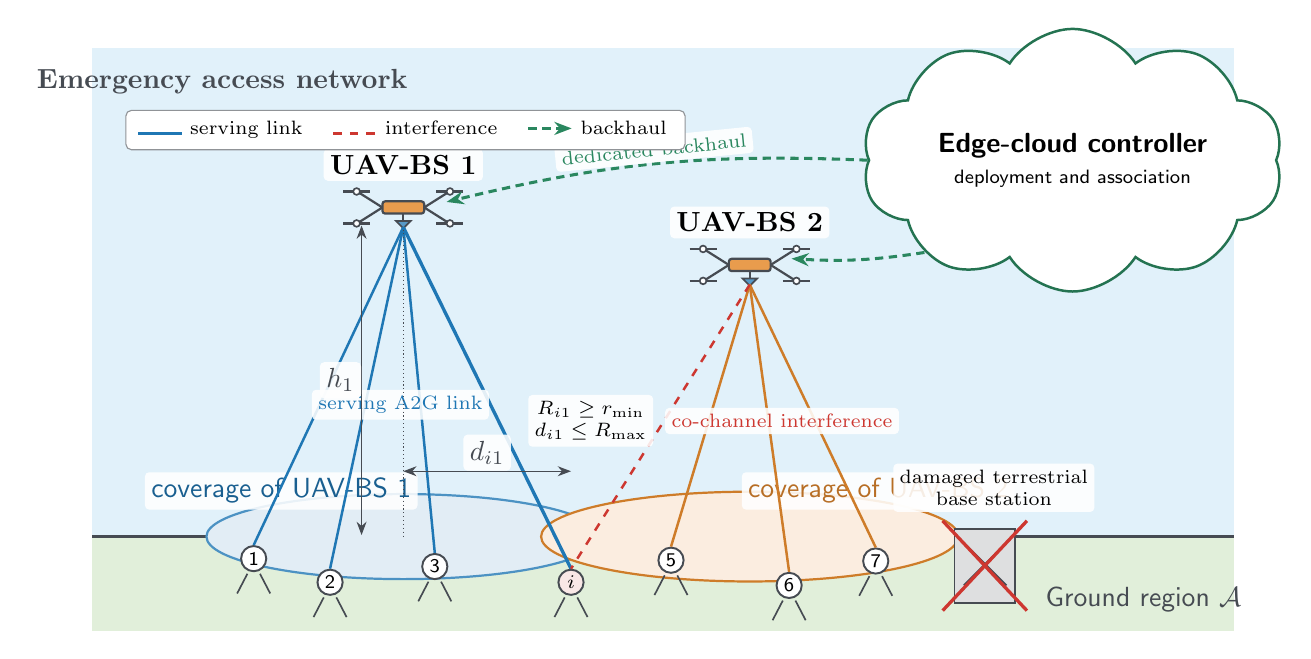
\begin{tikzpicture}[x=1cm,y=1cm,font=\sffamily]
  % Background and deployment region
  \fill[skyblue] (-0.3,1.0) rectangle (14.2,7.2);
  \fill[groundgreen] (-0.3,-0.2) rectangle (14.2,1.0);
  \draw[darkgray,line width=0.9pt] (-0.3,1.0)--(14.2,1.0);
  \node[darkgray,font=\bfseries] at (1.35,6.78) {Emergency access network};
  \node[darkgray] at (13.05,0.20) {Ground region $\mathcal A$};

  % Coverage footprints
  \fill[accessblue!13] (3.65,1.0) ellipse (2.50 and 0.54);
  \draw[accessblue!80,line width=0.8pt] (3.65,1.0) ellipse (2.50 and 0.54);
  \fill[uavorange!15] (8.05,1.0) ellipse (2.65 and 0.57);
  \draw[uavorange!90!black,line width=0.8pt] (8.05,1.0) ellipse (2.65 and 0.57);
  \node[labelbox,text=accessblue!80!black] at (2.10,1.58)
    {coverage of UAV-BS 1};
  \node[labelbox,text=uavorange!80!black] at (9.68,1.58)
    {coverage of UAV-BS 2};

  % UAVs
  \uav{3.65}{5.18}{0.78}
  \uav{8.05}{4.45}{0.78}
  \node[labelbox,font=\bfseries] at (3.65,5.72) {UAV-BS 1};
  \node[labelbox,font=\bfseries] at (8.05,4.99) {UAV-BS 2};

  % Controller and backhaul
  \node[draw=backhaulgreen!85!black,fill=white,cloud,cloud puffs=10,
    cloud puff arc=115,aspect=2.0,minimum width=2.65cm,minimum height=1.12cm,
    align=center,line width=0.9pt] (cloud) at (12.15,5.78)
    {\bfseries Edge-cloud controller\\[-1pt]\scriptsize deployment and association};
  \draw[backhaul] (cloud.west) to[bend right=8]
    node[labelbox,above,sloped,font=\scriptsize] {dedicated backhaul} (4.20,5.25);
  \draw[backhaul] (cloud.south west) to[bend left=6] (8.58,4.53);

  % Users
  \node[user] (u1) at (1.75,0.72) {\scriptsize 1};
  \node[user] (u2) at (2.72,0.42) {\scriptsize 2};
  \node[user] (u3) at (4.05,0.62) {\scriptsize 3};
  \node[user,fill=interferencered!12] (ui) at (5.78,0.42) {\scriptsize $i$};
  \node[user] (u5) at (7.05,0.70) {\scriptsize 5};
  \node[user] (u6) at (8.55,0.38) {\scriptsize 6};
  \node[user] (u7) at (9.65,0.69) {\scriptsize 7};
  \foreach \u in {u1,u2,u3,ui,u5,u6,u7}{
    \draw[darkgray,line width=0.6pt] ($(\u.south)+(-0.08,-0.02)$)
      -- ++(-0.13,-0.25);
    \draw[darkgray,line width=0.6pt] ($(\u.south)+(0.08,-0.02)$)
      -- ++(0.13,-0.25);
  }

  % Serving access links
  \draw[access] (3.65,4.93)--(u1.north);
  \draw[access] (3.65,4.93)--(u2.north);
  \draw[access] (3.65,4.93)--(u3.north);
  \draw[access,line width=1.2pt] (3.65,4.93)--(ui.north)
    node[pos=0.52,labelbox,left,font=\scriptsize] {serving A2G link};
  \draw[uavorange!90!black,line width=0.9pt] (8.05,4.20)--(u5.north);
  \draw[uavorange!90!black,line width=0.9pt] (8.05,4.20)--(u6.north);
  \draw[uavorange!90!black,line width=0.9pt] (8.05,4.20)--(u7.north);

  % Interference in overlap
  \draw[interference] (8.05,4.20)--(ui.north)
    node[pos=0.48,labelbox,right,font=\scriptsize] {co-channel interference};

  % Dimensions and variables
  \draw[dimension] (3.12,1.02)--(3.12,4.95)
    node[midway,labelbox,left] {$h_1$};
  \draw[darkgray,densely dotted] (3.65,4.90)--(3.65,1.0);
  \draw[dimension] (3.65,1.83)--(5.78,1.83)
    node[midway,labelbox,above] {$d_{i1}$};
  \node[labelbox,align=center,font=\scriptsize] at (6.03,2.47)
    {$R_{i1}\ge r_{\min}$\\$d_{i1}\le R_{\max}$};

  % Damaged terrestrial infrastructure
  \draw[fill=darkgray!18,draw=darkgray,line width=0.7pt]
    (10.65,0.16) rectangle (11.42,1.10);
  \draw[darkgray,line width=0.7pt] (10.77,0.38)--(11.31,0.92)
    (10.77,0.92)--(11.31,0.38);
  \draw[interferencered,line width=1.2pt] (10.50,0.06)--(11.57,1.20)
    (10.50,1.20)--(11.57,0.06);
  \node[labelbox,align=center,font=\scriptsize] at (11.15,1.62)
    {damaged terrestrial\\base station};

  % Legend
  \node[draw=darkgray!60,fill=white,rounded corners=2pt,anchor=north west,
    inner sep=4pt,align=left,font=\scriptsize] at (0.12,6.42) {
      \tikz{\draw[access] (0,0)--(0.55,0);} serving link \quad
      \tikz{\draw[interference] (0,0)--(0.55,0);} interference \quad
      \tikz{\draw[backhaul] (0,0)--(0.55,0);} backhaul
  };
\end{tikzpicture}
\end{document}
